\documentclass[convert]{standalone}

\usepackage{tikz}
\pagestyle{empty}

% INT_AY22_L06_Fig01_Find_vec_comps.png

\begin{document}
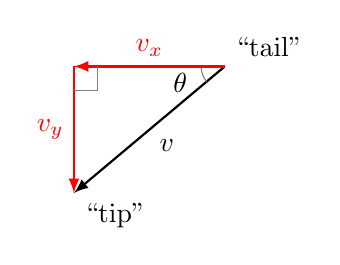
\begin{tikzpicture}[> = latex]

	% Definitions
	
	\def\Q{40}		% Size of angle for vector
	\def\M{2.5}		% Magnitude of vector
	\def\R{0.3}		% Radius of angle indicator arc, right angle indicator

	% Original vector w/ angle indicator
	
	\draw [thick, ->] (0, 0) node [above right] {``tail''}
		-- node [midway, below right] {$v$} (180 + \Q : \M) node [below right] {``tip''};
	\draw [thin, gray] (-\R, 0) arc (180 : 180 + \Q : \R);
	\draw [thin, gray, dashed] (0, 0) -- (-2 * \R, 0);
	\node at ({-2 * \R * cos(0.5 * \Q)}, {-2 * \R * sin(0.5 * \Q)}) {$\theta$};
	
	% Vector component arrows
	
	% These are added on later slides, as indicated by the number
	% given after the \draw command; important to have `->' for the
	% \draw commands, and to put double braces when trying to have
	% the node text be visible on a later slide
	
	\begin{scope}[thick, red, ->]
	
		\draw (0, 0) -- node [midway, above] {$v_x$} ({-\M * cos(\Q)}, 0);
		\draw ({-\M * cos(\Q)}, 0) -- node [midway, left] {$v_y$} ({-\M * cos(\Q)}, {-\M * sin(\Q)});
	
	\end{scope}
	
	% Right angle indicator
	
	\draw [thin, gray] ({-\M * cos(\Q) + \R}, 0) -- ++ (0, -\R) -- ++ (-\R, 0);

\end{tikzpicture}
\end{document}